\documentclass[t]{beamer}
%\mode<presentation>

\setbeamertemplate{itemize items}[circle]
\setbeamertemplate{headline}{% 
  \hfill% 
  \usebeamercolor[fg]{page number in head/foot}% 
  \usebeamerfont{page number in head/foot}% 
  \insertpagenumber% 
  \kern1em\vskip-1em% 
}
\usetheme{Antibes}
\usepackage{pgfpages}
%\setbeameroption{show notes}
%\setbeameroption{show notes on second screen=right}
\usepackage{apalike}
\usepackage{graphicx} % Required for including images
\graphicspath{{figures/}} % Location of the graphics files
\usepackage{booktabs} % Top and bottom rules for table
\usepackage[font=small,labelfont=bf]{caption} % Required for specifying captions to tables and figures
\usepackage{wrapfig} % Allows wrapping text around tables and figures
\usepackage{lipsum,adjustbox}
\usepackage[absolute,overlay]{textpos}
\usepackage{url}
\usepackage{lmodern}
\usepackage{amsmath}
\usepackage{amsfonts}
\usepackage{color}
\usepackage{array}
\usepackage{multirow}
\usepackage{multicol}
\usepackage{minibox}
\usepackage{tikz}
\usepackage{tikz-dependency}
\usepackage{algorithmic}
\usepackage{mathtools}
\usetikzlibrary{arrows.meta,graphs,graphs.standard,graphdrawing,quotes,shapes}
\usegdlibrary{layered,trees}
\tikzset{
  invisible/.style={opacity=0},
  visible on/.style={alt={#1{}{invisible}}},
  alt/.code args={<#1>#2#3}{%
    \alt<#1>{\pgfkeysalso{#2}}{\pgfkeysalso{#3}} % \pgfkeysalso doesn't change the path
  },
}
\captionsetup{labelformat=empty}
\DeclareMathOperator*{\argmin}{arg\,min}
\DeclareMathOperator*{\argmax}{arg\,max}

\makeatletter
\pgfdeclareshape{vector}{
	  \inheritsavedanchors[from={rectangle}]
	  \inheritbackgroundpath[from={rectangle}]
	  \inheritanchorborder[from={rectangle}]
	  \foreach \x in {center,north east,north west,north,south,south east,south west,east,west}{
	    \inheritanchor[from={rectangle}]{\x}
	  }

    \backgroundpath{
      \pgftransformshift{\pgfpoint{-16pt}{-4pt}}
		  \draw[rounded corners=2pt] (0,0) rectangle (32pt,8pt);
    }

    \beforebackgroundpath{
      \draw[step=8pt,help lines,-] (8pt,.1pt) grid (24pt,7.9pt);
    }
}
\makeatother

\AtBeginSection[]{
  \begin{frame}
  \vfill
  \centering
  \begin{beamercolorbox}[sep=8pt,center,shadow=true,rounded=true]{title}
    \usebeamerfont{title}\insertsectionhead\par%
  \end{beamercolorbox}
  \vfill
  \end{frame}
}

\title{Transition-based parsing}
\author{Daniel Hershcovich}
\date{Natural Language Processing, 67658 \\ December 24, 2017}

\begin{document}

\frame{\titlepage}

\frame{\frametitle{Overview}\tableofcontents} 


%----------------------------------------------------------------------------------------

\section{Introduction}

\begin{frame}
  \frametitle{Dependency parsing}
  Given sentence $w=(w_1, \ldots, w_n)$,
  let $V_w=\{0, 1, \ldots, n \}$ \\
  (the root node has index 0).
  
  Derive dependency tree $T=(V_w,A)$ by finding the set of arcs
  $A \subset V_w \times \mathcal{L} \times V_w$,
  where $\mathcal{L}$ is the set of possible edge labels.
  
  \vfill

  Equivalently---for each $i$, find $w_i$'s head and dependency label.
  
  \pause
  
  \begin{center}
	  \begin{minipage}{4cm}
	    $w=(w_1, w_2, w_3)$ \hfill $\Rightarrow$
	  \end{minipage}
	  \begin{minipage}{5cm}
	    \begin{dependency}
	      \begin{deptext}[column sep=1.5em,ampersand replacement=\^,font=\rmfamily]
	        $w_1$ \^ $w_2$ \^ $w_3$ \\
	      \end{deptext}
	      \deproot{2}{root}
	      \depedge{2}{1}{nsubj}
	      \depedge{2}{3}{dobj}
	    \end{dependency}
	  \end{minipage}
  \end{center}
  \[
      V_w=\{0,1,2,3\}, \quad
      A=\{(0,\mathrm{root},2),(2,\mathrm{nsubj},1),(2,\mathrm{dobj},3)\}
  \]
  
  \pause

  In transition-based parsing,
  the problem is decomposed to finding a sequence of \textit{transitions}.
\end{frame}

\begin{frame}
  \frametitle{Example}
    \scalebox{.6}{\begin{varwidth}{1.8\linewidth}
	\minibox[frame]{
	\begin{dependency}
	\begin{deptext}[column sep=.7cm]
	Alice \& saw \& Bob \\
	\end{deptext}
	\deproot[color=white]{2}{root}
	\end{dependency}
	\\
	\begin{tabular}{|l|}\hline
	\color{red} root \\ \hline
	\end{tabular}
	\hfill
	\begin{tabular}{|l|l|l|}
	\hline
	\color{blue} Alice & \color{blue} saw & \color{blue} Bob \\ \hline
	\end{tabular}
	}
	\begin{tabular}{c}\textsc{shift}\\$\rightarrow$\end{tabular}
	\minibox[frame]{
	\begin{dependency}
	\begin{deptext}[column sep=.7cm]
	Alice \& saw \& Bob \\
	\end{deptext}
	\deproot[color=white]{2}{root}
	\end{dependency}
	\\
	\begin{tabular}{|l|l|}\hline
	\color{red} root & \color{red} Alice \\ \hline
	\end{tabular}
	\hfill
	\begin{tabular}{|l|l|}\hline
	\color{blue} saw & \color{blue} Bob \\ \hline
	\end{tabular}
	}
	\begin{tabular}{c}\textsc{shift}\\$\rightarrow$\end{tabular}
	\minibox[frame]{
	\begin{dependency}
	\begin{deptext}[column sep=.7cm]
	Alice \& saw \& Bob \\
	\end{deptext}
	\deproot[color=white]{2}{root}
	\end{dependency}
	\\
	\begin{tabular}{|l|l|l|}\hline
	\color{red} root & \color{red} Alice & \color{red} saw \\ \hline
	\end{tabular}
	\hfill
	\begin{tabular}{|l|}\hline
	\color{blue} Bob \\ \hline
	\end{tabular}
	}
	\begin{tabular}{c}\textsc{left}\\ \textsc{arc}\\{\footnotesize nsubj}\\$\rightarrow$\end{tabular}

    \vspace{5mm}
	
	\minibox[frame]{
	\begin{dependency}
	\begin{deptext}[column sep=.7cm]
	Alice \& saw \& Bob \\
	\end{deptext}
	\deproot[color=white]{2}{root}
	\depedge{2}{1}{nsubj}
	\end{dependency}
	\\
	\begin{tabular}{|l|l|}\hline
	\color{red} root & \color{red} saw \\ \hline
	\end{tabular}
	\hspace{11mm}
	\begin{tabular}{|l|}\hline
	\color{blue} Bob \\ \hline
	\end{tabular}
	}
	\begin{tabular}{c}\textsc{shift}\\$\rightarrow$\end{tabular}
	\minibox[frame]{
	\begin{dependency}
	\begin{deptext}[column sep=.7cm]
	Alice \& saw \& Bob \\
	\end{deptext}
	\deproot[color=white]{2}{root}
	\depedge{2}{1}{nsubj}
	\end{dependency}
	\\
	\begin{tabular}{|l|l|l|} \hline
	\color{red} root & \color{red} saw & \color{red} Bob \\ \hline
	\end{tabular}
	\hspace{5.6mm}
	\begin{tabular}{|l|}\hline
	\quad \\ \hline
	\end{tabular}
	}
	\begin{tabular}{c}\textsc{right}\\ \textsc{arc}\\{\footnotesize dobj}\\$\rightarrow$\end{tabular}
	\minibox[frame]{
	\begin{dependency}
	\begin{deptext}[column sep=.7cm]
	Alice \& saw \& Bob \\
	\end{deptext}
	\deproot[color=white]{2}{root}
	\depedge{2}{1}{nsubj}
	\depedge{2}{3}{dobj}
	\end{dependency}
	\\
	\begin{tabular}{|l|l|}\hline
	\color{red} root & \color{red} saw \\ \hline
	\end{tabular}
	\hspace{16mm}
	\begin{tabular}{|l|}\hline
	\quad \\ \hline
	\end{tabular}
	}
	\begin{tabular}{c}\textsc{right}\\ \textsc{arc}\\{\footnotesize root}\\$\rightarrow$\end{tabular}
	
    \vspace{5mm}
	
	\minibox[frame]{
	\begin{dependency}
	\begin{deptext}[column sep=.7cm]
	Alice \& saw \& Bob \\
	\end{deptext}
	\deproot{2}{root}
	\depedge{2}{1}{nsubj}
	\depedge{2}{3}{dobj}
	\end{dependency}
	\\
	\begin{tabular}{|l|l|}\hline
	\color{red} root \\ \hline
	\end{tabular}
	\hspace{27mm}
	\begin{tabular}{|l|}\hline
	\quad \\ \hline
	\end{tabular}
	}
    \end{varwidth}
	}
\end{frame}

\section{Transition systems}

\begin{frame}
  \frametitle{Configurations}
  Transitions operate on the parser \textit{configuration} (or \textit{state})
  \[
    c = (\Sigma, B, A)
  \]
  where
  \begin{itemize}
    \item $\Sigma \subseteq V_w$ is the stack of partially processed items.
    \item $B \subseteq V_w$ is the buffer of remaining input tokens.
    \item $A \subset V_w \times \mathcal{L} \times V_w$ is the set of arcs constructed so far.
  \end{itemize}
  
  \pause\vfill
  
  Common notation:
  \begin{equation*}
  \begin{split}
      \Sigma&=[\ldots,s_1,s_0]=\Sigma^\prime|s_1|s_0 \\
      B&=[b_0,b_1,\ldots]=b_0|b_1|B^\prime
  \end{split}
  \end{equation*}
\end{frame}

\begin{frame}
  \frametitle{Transition systems}  
  
  A \textit{transition system} is defined as
  \[
    S = (\mathcal{C}, \mathcal{T}, c_s, C_t)
  \]
  where
  \begin{itemize}
    \item $\mathcal{C}$ is the set of possible configurations.
    \item $\mathcal{T} \subset \mathcal{C}^\mathcal{C}$ is the set of \textit{transitions}.
    \item $c_s$ maps every sentence $w$ to an initial configuration $c_s(w)$.
    \item $C_t \subset \mathcal{C}$ is the set of terminal configurations.
  \end{itemize}
\end{frame}

\begin{frame}
  \frametitle{Transition sequence}  
  A \textit{transition sequence} is $(c_0, \ldots, c_m) \subseteq \mathcal{C}$ s.t.
  \begin{itemize}
    \item $c_0 = c_s(w)$
    \item $c_m = (\Sigma_m, B_m, A_m) \in C_t$
    \item For each $i=1,\ldots,m$ there exists $t\in \mathcal{T}$ s.t. $c_{i+1}=t(c_i)$.
  \end{itemize}
  
  The output of the system is then $T=(V_w,A_m)$.
\end{frame}

\begin{frame}
  \frametitle{Arc-standard transition system \cite{nivre2004incrementality}}
  Transition set $\mathcal{T}$:

  \begin{tabular}{ll}
    $\textsc{shift}$ & move one item from the buffer to the stack: \\
    & $(\Sigma, \; i | B, \; A) \Rightarrow (\Sigma | i, \; B, \; A)$ \\
    \hline
    $\textsc{left-arc}_\ell$ & create arc $s_0 \to s_1$ with label $\ell \in \mathcal{L}$ and remove $s_1$: \\
    & $(\Sigma | i|j, \; B, \; A) \Rightarrow (\Sigma | j, \; B, \; A \cup \{(j,\ell,i)\})$ \\
    & Condition: $i\neq0$ \\
    \hline
    $\textsc{right-arc}_\ell$ & create arc $s_1 \to s_0$ with label $\ell \in \mathcal{L}$ and remove $s_0$: \\
    & $(\Sigma | i|j, \; B, \; A) \Rightarrow (\Sigma | i, \; B, \; A \cup \{(i,\ell,j)\})$  
  \end{tabular}
  
  \pause\vfill
  
  Typically $|\mathcal{L}| \approx 50$,
  so there are 101 different transitions.

  \pause\vfill

  Initial configuration:
  \[
    c_s(w_1, w_2, w_3, \ldots,) = ([0], [1, 2, 3, \ldots], \emptyset)
  \]

  Terminal configuration:
  \[
    c_t = ([0], [], A)
  \]
\end{frame}

\begin{frame}
  \frametitle{Properties of the arc-standard system
  \footnotetext[1]{\url{http://aclweb.org/anthology/J08-4003}}}
  \begin{description}
  \item[Soundness.] Every transition sequence outputs a projective tree.
  \item[Completeness.] Every projective tree is output by some sequence.
  \item[Complexity.] Input of length $n$ requires exactly $2n$ transitions.
  \item[Bottom-up.] Attaches a token's head only after all dependents.
  \end{description}
\end{frame}

\begin{frame}
    \frametitle{Projectivity}
    Projective tree (no crossing arcs $\Leftrightarrow$ all sub-trees are sub-strings):
  \begin{center}
	\begin{dependency}
	\begin{deptext}[column sep=.7cm]
	Alice \& saw \& Bob \\
	\end{deptext}
	\deproot{2}{root}
	\depedge{2}{1}{nsubj}
	\depedge{2}{3}{dobj}
	\end{dependency}
	\end{center}
	
	Non-projective tree (cannot be parsed by arc-standard):
  \begin{center}
    \begin{dependency}
      \begin{deptext}[column sep=1.5em,ampersand replacement=\^,font=\rmfamily]
        That \^ 's \^ what \^ they \^ 're \^ after \\
      \end{deptext}
      \depedge{2}{1}{nsubj}
      \deproot{2}{root}
      \depedge[edge start x offset=.75em]{6}{3}{pobj}
      \depedge{5}{4}{nsubj}
      \depedge[edge unit distance=.75em]{2}{5}{ccomp}
      \depedge{5}{6}{prep}
    \end{dependency}
  \end{center}
\end{frame}

\begin{frame}
  \frametitle{Another example for arc-standard transition sequence}
    \scalebox{.5}{\begin{varwidth}{2.2\linewidth}
	\minibox[frame]{
	\begin{dependency}
	\begin{deptext}[column sep=.7cm]
	Alice \& looked \& at \& Bob \\
	\end{deptext}
	\deproot[color=white]{2}{root}
	\end{dependency}
	\\
	\begin{tabular}{|l|}\hline
	\color{red} root \\ \hline
	\end{tabular}
	\hfill
	\begin{tabular}{|l|l|l|l|}
	\hline
	\color{blue} Alice & \color{blue} looked & \color{blue} at & \color{blue} Bob \\ \hline
	\end{tabular}
	}
	\begin{tabular}{c}\textsc{shift}\\$\rightarrow$\end{tabular}
	\minibox[frame]{
	\begin{dependency}
	\begin{deptext}[column sep=.7cm]
	Alice \& looked \& at \& Bob \\
	\end{deptext}
	\deproot[color=white]{2}{root}
	\end{dependency}
	\\
	\begin{tabular}{|l|l|}\hline
	\color{red} root & \color{red} Alice \\ \hline
	\end{tabular}
	\hfill
	\begin{tabular}{|l|l|l|}\hline
	\color{blue} looked & \color{blue} at & \color{blue} Bob \\ \hline
	\end{tabular}
	}
	\begin{tabular}{c}\textsc{shift}\\$\rightarrow$\end{tabular}
	\minibox[frame]{
	\begin{dependency}
	\begin{deptext}[column sep=.7cm]
	Alice \& looked \& at \& Bob \\
	\end{deptext}
	\deproot[color=white]{2}{root}
	\end{dependency}
	\\
	\begin{tabular}{|l|l|l|}\hline
	\color{red} root & \color{red} Alice & \color{red} looked \\ \hline
	\end{tabular}
	\hfill
	\begin{tabular}{|l|l|}\hline
	\color{blue} at & \color{blue} Bob \\ \hline
	\end{tabular}
	}
	\begin{tabular}{c}\textsc{left}\\ \textsc{arc}\\{\footnotesize nsubj}\\$\rightarrow$\end{tabular}

    \vspace{5mm}
	
	\minibox[frame]{
	\begin{dependency}
	\begin{deptext}[column sep=.7cm]
	Alice \& looked \& at \& Bob \\
	\end{deptext}
	\deproot[color=white]{2}{root}
	\depedge{2}{1}{nsubj}
	\end{dependency}
	\\
	\begin{tabular}{|l|l|}\hline
	\color{red} root & \color{red} looked \\ \hline
	\end{tabular}
	\hspace{11mm}
	\begin{tabular}{|l|l|}\hline
	\color{blue} at & \color{blue} Bob \\ \hline
	\end{tabular}
	}
	\begin{tabular}{c}\textsc{shift}\\$\rightarrow$\end{tabular}
	\minibox[frame]{
	\begin{dependency}
	\begin{deptext}[column sep=.7cm]
	Alice \& looked \& at \& Bob \\
	\end{deptext}
	\deproot[color=white]{2}{root}
	\depedge{2}{1}{nsubj}
	\end{dependency}
	\\
	\begin{tabular}{|l|l|l|} \hline
	\color{red} root & \color{red} looked & \color{red} at \\ \hline
	\end{tabular}
	\hspace{11mm}
	\begin{tabular}{|l|}\hline
	\color{blue} Bob \\ \hline
	\end{tabular}
	}
	\begin{tabular}{c}\textsc{shift}\\$\rightarrow$\end{tabular}
	\minibox[frame]{
	\begin{dependency}
	\begin{deptext}[column sep=.7cm]
	Alice \& looked \& at \& Bob \\
	\end{deptext}
	\deproot[color=white]{2}{root}
	\depedge{2}{1}{nsubj}
	\end{dependency}
	\\
	\begin{tabular}{|l|l|l|l|}\hline
	\color{red} root & \color{red} looked & \color{red} at & \color{red} Bob \\ \hline
	\end{tabular}
	\hspace{6mm}
	\begin{tabular}{|l|}\hline
	\quad \\ \hline
	\end{tabular}
	}
	\begin{tabular}{c}\textsc{right}\\ \textsc{arc}\\{\footnotesize pobj}\\$\rightarrow$\end{tabular}
	
    \vspace{5mm}
	
	\minibox[frame]{
	\begin{dependency}
	\begin{deptext}[column sep=.7cm]
	Alice \& looked \& at \& Bob \\
	\end{deptext}
	\deproot[color=white]{2}{root}
	\depedge{2}{1}{nsubj}
	\depedge{3}{4}{pobj}
	\end{dependency}
	\\
	\begin{tabular}{|l|l|l|} \hline
	\color{red} root & \color{red} looked & \color{red} at \\ \hline
	\end{tabular}
	\hspace{17mm}
	\begin{tabular}{|l|}\hline
	\quad \\ \hline
	\end{tabular}
	}
	\begin{tabular}{c}\textsc{right}\\ \textsc{arc}\\{\footnotesize prep}\\$\rightarrow$\end{tabular}
	\minibox[frame]{
	\begin{dependency}
	\begin{deptext}[column sep=.7cm]
	Alice \& looked \& at \& Bob \\
	\end{deptext}
	\deproot[color=white]{2}{root}
	\depedge{2}{1}{nsubj}
	\depedge{2}{3}{prep}
	\depedge{3}{4}{pobj}
	\end{dependency}
	\\
	\begin{tabular}{|l|l|l|}\hline
	\color{red} root & \color{red} looked \\ \hline
	\end{tabular}
	\hspace{25mm}
	\begin{tabular}{|l|}\hline
	\quad \\ \hline
	\end{tabular}
	}
	\begin{tabular}{c}\textsc{right}\\ \textsc{arc}\\{\footnotesize root}\\$\rightarrow$\end{tabular}
	\minibox[frame]{
	\begin{dependency}
	\begin{deptext}[column sep=.7cm]
	Alice \& looked \& at \& Bob \\
	\end{deptext}
	\deproot{2}{root}
	\depedge{2}{1}{nsubj}
	\depedge{2}{3}{prep}
	\depedge{3}{4}{pobj}
	\end{dependency}
	\\
	\begin{tabular}{|l|l|}\hline
	\color{red} root \\ \hline
	\end{tabular}
	\hspace{40mm}
	\begin{tabular}{|l|}\hline
	\quad \\ \hline
	\end{tabular}
	}
    \end{varwidth}
	}
	
	\pause\vfill
	Might be a good idea to attach $\textrm{looked} \to \textrm{at}$ as soon as possible?
\end{frame}


\begin{frame}
  \frametitle{Arc-eager transition system \cite{nivre2004incrementality}}
  \begin{tabular}{ll}
    $\textsc{shift}$ & move one item from the buffer to the stack: \\
    (same) & $(\Sigma, \; i | B, \; A) \Rightarrow (\Sigma | i, \; B, \; A)$ \\
    \hline
    $\textsc{left-arc}_\ell$ & create arc $b_0 \to s_0$ with label $\ell \in \mathcal{L}$ and remove $s_0$: \\
    & $(\Sigma | i, \; j | B, \; A) \Rightarrow (\Sigma, \; j | B, \; A \cup \{(j,\ell,i)\})$ \\
    & Condition: $i\neq0$ and $i$ has no head \\
    \hline
    $\textsc{right-arc}_\ell$ & create arc $s_0 \to b_0$ with label $\ell \in \mathcal{L}$ and shift $b_0$: \\
    & $(\Sigma | i, \; j | B, \; A) \Rightarrow (\Sigma | i|j, \; B, \; A \cup \{(i,\ell,j)\})$   \\
    \hline
    $\textsc{reduce}$ & remove $s_0$: \\
    & $(\Sigma | i, \; B, \; A) \Rightarrow (\Sigma, \; B, \; A)$ \\
    & Condition: $i$ has a head
  \end{tabular}
  
  \pause\vfill

  Initial configuration: same as arc-standard.

  Terminal configuration ($\Sigma$ does not have to be $[0]$):
  \[
    c_t = (\Sigma, [], A)
  \]
\end{frame}

\begin{frame}
  \frametitle{Properties of the arc-eager system}
  Soundness and completeness are the same as arc-standard.
  
  Complexity: \textbf{at most} $2n$.
  
  \pause\vfill
  
  Builds left-dependents bottom-up and right-dependents top-down.
  Increased incrementality---no need to wait for the whole sub-tree to be complete before attaching it.
  
  \vfill
  
  \begin{center}
  \scalebox{.6}{
    \begin{dependency}
	\begin{deptext}[column sep=.7cm]
	Alice \& looked \& at \& the \& quiet \& old \& man \& who \& sat \& in \& the \& corner \\
	\end{deptext}
	\deproot{2}{root}
	\depedge{2}{1}{nsubj}
	\depedge[color=red]{2}{3}{prep}
	\end{dependency}
	}
  \end{center}
\end{frame}

\begin{frame}
  \frametitle{Example arc-eager transition sequence}
    \scalebox{.5}{\begin{varwidth}{2.2\linewidth}
	\minibox[frame]{
	\begin{dependency}
	\begin{deptext}[column sep=.7cm]
	Alice \& looked \& at \& Bob \\
	\end{deptext}
	\deproot[color=white]{2}{root}
	\end{dependency}
	\\
	\begin{tabular}{|l|}\hline
	\color{red} root \\ \hline
	\end{tabular}
	\hfill
	\begin{tabular}{|l|l|l|l|}
	\hline
	\color{blue} Alice & \color{blue} looked & \color{blue} at & \color{blue} Bob \\ \hline
	\end{tabular}
	}
	\begin{tabular}{c}\textsc{shift}\\$\rightarrow$\end{tabular}
	\minibox[frame]{
	\begin{dependency}
	\begin{deptext}[column sep=.7cm]
	Alice \& looked \& at \& Bob \\
	\end{deptext}
	\deproot[color=white]{2}{root}
	\end{dependency}
	\\
	\begin{tabular}{|l|l|}\hline
	\color{red} root & \color{red} Alice \\ \hline
	\end{tabular}
	\hfill
	\begin{tabular}{|l|l|l|}\hline
	\color{blue} looked & \color{blue} at & \color{blue} Bob \\ \hline
	\end{tabular}
	}
	\begin{tabular}{c}\textsc{left}\\ \textsc{arc}\\{\footnotesize nsubj}\\$\rightarrow$\end{tabular}
	\minibox[frame]{
	\begin{dependency}
	\begin{deptext}[column sep=.7cm]
	Alice \& looked \& at \& Bob \\
	\end{deptext}
	\deproot[color=white]{2}{root}
	\depedge{2}{1}{nsubj}
	\end{dependency}
	\\
	\begin{tabular}{|l|}\hline
	\color{red} root \\ \hline
	\end{tabular}
	\hfill
	\begin{tabular}{|l|l|l|}\hline
	\color{blue} looked & \color{blue} at & \color{blue} Bob \\ \hline
	\end{tabular}
	}
	\begin{tabular}{c}\textsc{right}\\ \textsc{arc}\\{\footnotesize root}\\$\rightarrow$\end{tabular}

    \vspace{5mm}
	
	\minibox[frame]{
	\begin{dependency}
	\begin{deptext}[column sep=.7cm]
	Alice \& looked \& at \& Bob \\
	\end{deptext}
	\deproot{2}{root}
	\depedge{2}{1}{nsubj}
	\end{dependency}
	\\
	\begin{tabular}{|l|l|}\hline
	\color{red} root & \color{red} looked \\ \hline
	\end{tabular}
	\hspace{11mm}
	\begin{tabular}{|l|l|}\hline
	\color{blue} at & \color{blue} Bob \\ \hline
	\end{tabular}
	}
	\begin{tabular}{c}\textsc{right}\\ \textsc{arc}\\{\footnotesize prep}\\$\rightarrow$\end{tabular}
	\minibox[frame]{
	\begin{dependency}
	\begin{deptext}[column sep=.7cm]
	Alice \& looked \& at \& Bob \\
	\end{deptext}
	\deproot{2}{root}
	\depedge{2}{1}{nsubj}
	\depedge{2}{3}{prep}
	\end{dependency}
	\\
	\begin{tabular}{|l|l|l|} \hline
	\color{red} root & \color{red} looked & \color{red} at \\ \hline
	\end{tabular}
	\hspace{11mm}
	\begin{tabular}{|l|}\hline
	\color{blue} Bob \\ \hline
	\end{tabular}
	}
	\begin{tabular}{c}\textsc{right}\\ \textsc{arc}\\{\footnotesize pobj}\\$\rightarrow$\end{tabular}
	\minibox[frame]{
	\begin{dependency}
	\begin{deptext}[column sep=.7cm]
	Alice \& looked \& at \& Bob \\
	\end{deptext}
	\deproot{2}{root}
	\depedge{2}{1}{nsubj}
	\depedge{2}{3}{prep}
	\depedge{3}{4}{pobj}
	\end{dependency}
	\\
	\begin{tabular}{|l|l|l|l|}\hline
	\color{red} root & \color{red} looked & \color{red} at & \color{red} Bob \\ \hline
	\end{tabular}
	\hspace{6mm}
	\begin{tabular}{|l|}\hline
	\quad \\ \hline
	\end{tabular}
	}
    \end{varwidth}
	}
\end{frame}

\section{Greedy transition-based parsing}

\begin{frame}
  \frametitle{Transition-based (shift-reduce) parsing}
    To actually parse text, we need to decide which transitions to take.
    \[
        P(t_1,\ldots,t_m|w)=\prod_{i=1}^mP(t_i|t_1,\ldots,t_{i-1},w)=\prod_{i=1}^mP(t_i|c_{i-1})
    \]
    so inference is
    \[
    \argmax_{t_1,\ldots,t_m \in \mathcal{T}} \prod_{i=1}^mP(t_i|c_{i-1})
    \]

    But training examples are trees, not sequences.
    
    To learn this score, we need an \textit{oracle} to tell the correct sequence:
    \[
    o(T)=(t_1,\ldots,t_m)
    \]
    
    \pause\vfill
    
    \centering
    \scalebox{.7}{
    \begin{minipage}{.4\textwidth}
	\begin{dependency}
	\begin{deptext}[column sep=.7cm]
	Alice \& saw \& Bob \\
	\end{deptext}
	\deproot{2}{root}
	\depedge{2}{1}{nsubj}
	\depedge{2}{3}{dobj}
	\end{dependency}
	\end{minipage}
    \begin{minipage}{.05\textwidth}
	$\Rightarrow$
	\end{minipage}
    \begin{minipage}{1.2\textwidth}
    $\textsc{shift},
	\textsc{shift},
	\textsc{left-arc}_\mathrm{nsubj},
	\textsc{shift},
	\textsc{right-arc}_\mathrm{dobj},
	\textsc{right-arc}_\mathrm{root}$
	\end{minipage}
	}
\end{frame}

\begin{frame}
    \frametitle{Oracle for arc-standard}
    \begin{algorithmic}[0]
    \WHILE{$B\neq[]$ and $\Sigma\neq[0]$}
        \IF{$s_0\xrightarrow{\ell} s_1$ and $s_1$ has all its children and $s_1\neq0$}
            \RETURN $\textsc{left-arc}_\ell$
        \ELSIF{$s_1\xrightarrow{\ell} s_0$ and $s_0$ has all its children and $s_0\neq0$}
            \RETURN $\textsc{right-arc}_\ell$
        \ELSE
            \RETURN $\textsc{shift}$
        \ENDIF
    \ENDWHILE
    \end{algorithmic}
\end{frame}

\begin{frame}
    \frametitle{Oracle for arc-eager}
    \begin{algorithmic}[0]
    \WHILE{$B\neq[]$}
        \IF{$b_0\xrightarrow{\ell} s_0$}
            \RETURN $\textsc{left-arc}_\ell$
        \ELSIF{$s_0\xrightarrow{\ell} b_0$}
            \RETURN $\textsc{right-arc}_\ell$
        \ELSIF{$s_0$ has all its children and a head}
            \RETURN $\textsc{reduce}$
        \ELSE
            \RETURN $\textsc{shift}$
        \ENDIF
    \ENDWHILE
    \end{algorithmic}
\end{frame}

\begin{frame}
    \frametitle{Greedy transition-based parsing}
    In \textit{greedy parsing}, instead of
    \[
    (t_1,\ldots,t_m)=\argmax_{t^\prime_1,\ldots,t^\prime_m \in \mathcal{T}} \prod_{i=1}^mP(t^\prime_i|c_{i-1})
    \]
    we select each transition separately and sequentially:
    \[
    t_i = \argmax_{t^\prime_i \in \mathcal{T}} P(t^\prime_i|c_{i-1}) \quad i=1,\ldots,m
    \]
    
    \pause
    
    A score $s(t, c)$ estimates this probability. Parsing algorithm:
    
    \begin{algorithmic}[0]
    \STATE{$c\leftarrow c_s(w)$}
    \WHILE{$c\not\in C_t$}
        \STATE{$c\leftarrow\Big(\argmax_{t\in\mathcal{T}}s(t,c)\Big)(c)$}
    \ENDWHILE
    \end{algorithmic}
\end{frame}

\begin{frame}
    \frametitle{Transition classifiers}
    Learn the score giving maximum probability to oracle transitions:
    \[
    \argmax_{s\in\mathcal{S}}\sum_{i=1}^ms(t^*_i,c^*_{i-1})
    \]
    where $t^*_1,\ldots,t^*_m$ (and $c^*_1,\ldots,c^*_m$) are determined by the oracle.
    
    \pause\vfill
    
    Possible hypothesis classes $\mathcal{S}$:
    \begin{enumerate}
    \item Linear (perceptron)
    \item Feedforward neural networks
    \item Recurrent neural networks (RNN, LSTM, GRU)
    \end{enumerate}
    And others, e.g. SVM.
\end{frame}

\begin{frame}
    \frametitle{Linear transition classifier \cite{Nivre03anefficient}}
    Given features $\mathbf{f}=(f_1, \ldots, f_K) : \mathcal{C}\to\mathbb{R}^K$, learn weights $W_{|\mathcal{T}|\times K}$:
    \[
    s(t,c)=\big[W\cdot\mathbf{f}(c)\big]_t
    \]
    Typically trained by the perceptron algorithm, with binary features:
	words, POS and existing arc labels of stack and buffer nodes, and
	their heads and dependents.
\end{frame}

\begin{frame}
    \frametitle{NN transition classifier \cite{chen2014fast}}
    Dense \textbf{embedding} features instead of sparse binary features.
    Trained with backpropagation and stochastic gradient descent.
    
    \vfill
    
    Feedforward NN architecture:
    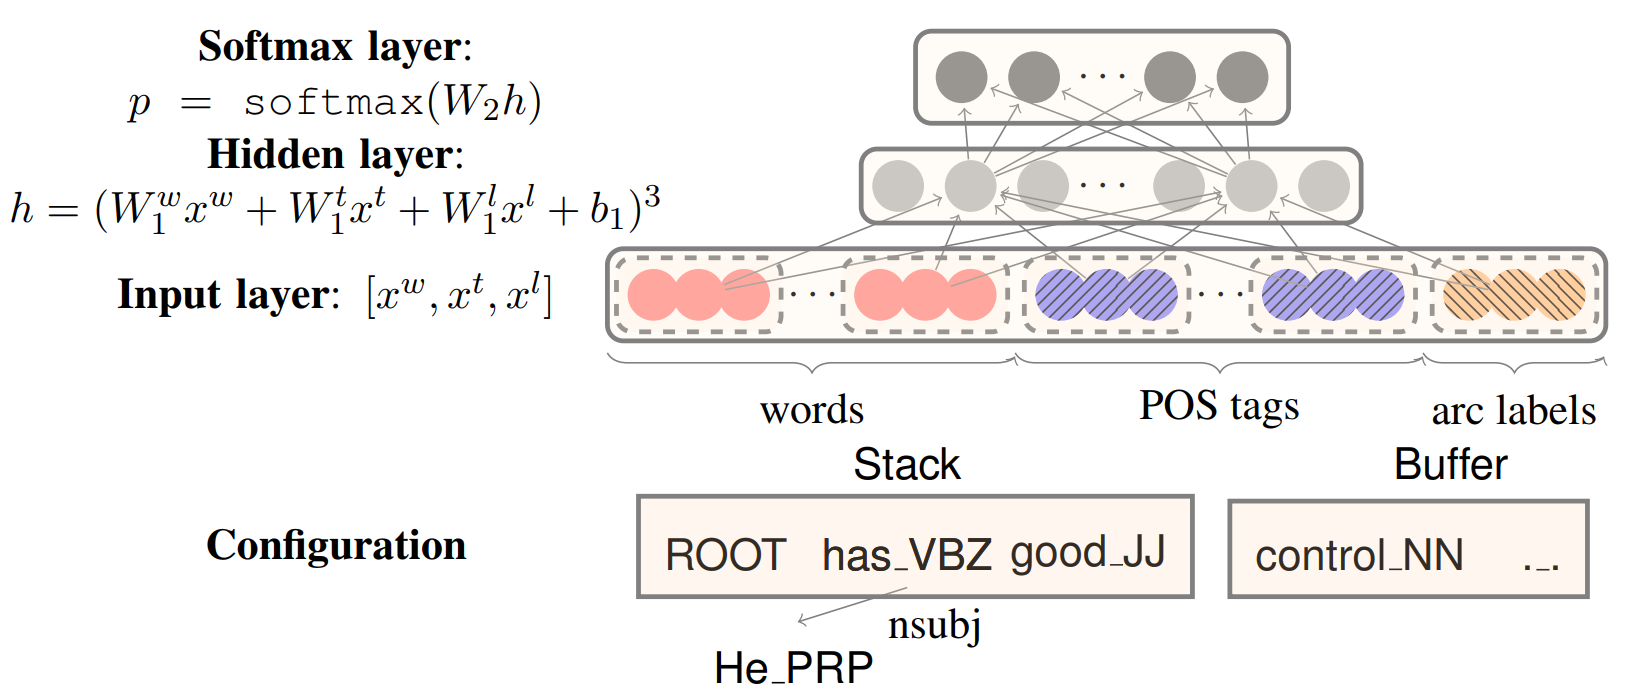
\includegraphics[width=\textwidth,height=\textheight,keepaspectratio]{nn.png}
\end{frame}

\begin{frame}
    \frametitle{Bi-RNN encoder \cite{kiperwasser2016simple}}
    Deep bidirectional LSTM RNN for input representations.
    
    \centering
    \scalebox{.85}{
	\begin{tikzpicture}[->]
	\tiny
	\tikzstyle{main}=[ellipse, minimum size=7mm, draw=black!80, node distance=12mm]
	\foreach \i/\word in {1/{John},3/{looked},5/{at},7/{Mary}} {
	    \uncover<1->{\node (x\i) at (\i,-1.3) {\small \word};}
	    \uncover<1->{\node[main, fill=white!100] (h\i) at (\i,0) {\textsc{lstm}};}
        \uncover<1->{\path (x\i) edge node[left]{\textit{embedding}} (h\i);}
	    \uncover<2->{\node[main, fill=white!100] (i\i) at (\i.5,.8) {\textsc{lstm}};}
        \uncover<2->{\path (x\i) edge [bend right] node[right]{\textit{embedding}} (i\i);}
	    \uncover<3->{\node[main, fill=white!100] (l\i) at (\i.5,2.3) {\textsc{lstm}};}
        \uncover<3->{\path (h\i) edge [bend left] (l\i);}
        \uncover<3->{\path (i\i) edge (l\i);}
	    \uncover<4->{\node[main, fill=white!100] (k\i) at (\i,3.1) {\textsc{lstm}};}
        \uncover<4->{\path (i\i) edge [bend left] (k\i);}
        \uncover<4->{\path (h\i) edge [bend left] (k\i);}
	}
	\uncover<3->{\node (l4) at (4.5,2.3) {\ldots};}
    \uncover<4->{\node (k4) at (4,3.1) {\ldots};}
    \uncover<2->{\node (i4) at (4.5,.8) {\ldots};}
    \uncover<1->{\node (h4) at (4,0) {\ldots};}
    \uncover<1->{\node (x4) at (4,-1.3) {\ldots};}
	\foreach \current/\next in {1/3,3/4,4/5,5/7} {
        \uncover<2->{\path (i\next) edge (i\current);}
        \uncover<1->{\path (h\current) edge (h\next);}
        \uncover<4->{\path (k\next) edge (k\current);}
        \uncover<3->{\path (l\current) edge (l\next);}
	}
	\uncover<5->{
        \node[main, fill=white!100] (mlp) at (4,4.6) {feedforward NN};
		\foreach \i in {1,3} {
	        \path (l\i) edge (mlp);
	        \path (k\i) edge (mlp);
	    }
	    \node (transition) at (4,5.8) {score};
	    \path (mlp) edge node[right] {\textit{softmax}} (transition);
    }
	\end{tikzpicture}
	}
\end{frame}

\begin{frame}
    \frametitle{Empirical comparison}
    Evaluation on PTB-SD\footnote{Penn Treebank Wall-Street Journal (WSJ) with Stanford Dependencies}:
    \begin{center}
    \begin{tabular}{l|cc}
    & UAS & LAS \\ \hline
    \small Graph-based \\
    MSTParser & 90.7 & 87.6 \\
    \hline
    \small Transition-based \\
    Linear \cite{ZhangTDP11} & 89.6 & 87.4 \\
    Feedforward NN \cite{chen2014fast} & 91.8 & 89.6 \\
    BiLSTM \cite{kiperwasser2016simple} & 93.9 & 91.9
    \end{tabular}
    \end{center}
\end{frame}

\section{Dealing with error propagation}

\begin{frame}
    \frametitle{Error propagation}
    Greedy transition-based parsers do not recover well from errors.
    \begin{center}
    \begin{dependency}
	\begin{deptext}[column sep=.7cm]
	Students \& sleep \& in \& class \\
	\end{deptext}
	\deproot{2}{root}
	\depedge{2}{1}{nsubj}
	\depedge{2}{3}{prep}
	\depedge{3}{4}{pobj}
	\end{dependency}
    \begin{dependency}
	\begin{deptext}[column sep=.7cm]
	Students \& sleep \& in \& often \\
	\end{deptext}
	\deproot{2}{root}
	\depedge{2}{1}{nsubj}
	\depedge{2}{3}{advmod}
	\depedge{2}{4}{advmod}
	\end{dependency}
    \end{center}
\end{frame}

\begin{frame}
    \frametitle{Error propagation example}
    Correct parse:
    
    \scalebox{.475}{\begin{varwidth}{2.3\linewidth}
	\minibox[frame]{
	\begin{dependency}
	\begin{deptext}[column sep=.7cm]
	Students \& sleep \& in \& class \\
	\end{deptext}
	\deproot[color=white]{2}{root}
	\end{dependency}
	\\
	\begin{tabular}{|l|}\hline
	\color{red} root \\ \hline
	\end{tabular}
	\hfill
	\begin{tabular}{|l|l|l|l|}
	\hline
	\color{blue} Students & \color{blue} sleep & \color{blue} in & \color{blue} class \\ \hline
	\end{tabular}
	}
	\begin{tabular}{c}\textsc{shift}\\$\rightarrow$\end{tabular}
	\minibox[frame]{
	\begin{dependency}
	\begin{deptext}[column sep=.7cm]
	Students \& sleep \& in \& class \\
	\end{deptext}
	\deproot[color=white]{2}{root}
	\end{dependency}
	\\
	\begin{tabular}{|l|l|}\hline
	\color{red} root & \color{red} Students \\ \hline
	\end{tabular}
	\hfill
	\begin{tabular}{|l|l|l|}\hline
	\color{blue} sleep & \color{blue} in & \color{blue} class \\ \hline
	\end{tabular}
	}
	\begin{tabular}{c}\textsc{shift}\\$\rightarrow$\end{tabular}
	\minibox[frame]{
	\begin{dependency}
	\begin{deptext}[column sep=.7cm]
	Students \& sleep \& in \& class \\
	\end{deptext}
	\deproot[color=white]{2}{root}
	\end{dependency}
	\\
	\begin{tabular}{|l|l|l|}\hline
	\color{red} root & \color{red} Students & \color{red} sleep \\ \hline
	\end{tabular}
	\hfill
	\begin{tabular}{|l|l|}\hline
	\color{blue} in & \color{blue} class \\ \hline
	\end{tabular}
	}
	\begin{tabular}{c}\textsc{left}\\ \textsc{arc}\\{\footnotesize nsubj}\\$\rightarrow$\end{tabular}

    \vspace{5mm}
	
	\minibox[frame]{
	\begin{dependency}
	\begin{deptext}[column sep=.7cm]
	Students \& sleep \& in \& class \\
	\end{deptext}
	\deproot[color=white]{2}{root}
	\depedge{2}{1}{nsubj}
	\end{dependency}
	\\
	\begin{tabular}{|l|l|}\hline
	\color{red} root & \color{red} sleep \\ \hline
	\end{tabular}
	\hspace{18mm}
	\begin{tabular}{|l|l|}\hline
	\color{blue} in & \color{blue} class \\ \hline
	\end{tabular}
	}
	\begin{tabular}{c}\textsc{shift}\\$\rightarrow$\end{tabular}
	\minibox[frame]{
	\begin{dependency}
	\begin{deptext}[column sep=.7cm]
	Students \& sleep \& in \& class \\
	\end{deptext}
	\deproot[color=white]{2}{root}
	\depedge{2}{1}{nsubj}
	\end{dependency}
	\\
	\begin{tabular}{|l|l|l|} \hline
	\color{red} root & \color{red} sleep & \color{red} in \\ \hline
	\end{tabular}
	\hspace{17mm}
	\begin{tabular}{|l|}\hline
	\color{blue} class \\ \hline
	\end{tabular}
	}
	\begin{tabular}{c}\textsc{shift}\\$\rightarrow$\end{tabular}
	\minibox[frame]{
	\begin{dependency}
	\begin{deptext}[column sep=.7cm]
	Students \& sleep \& in \& class \\
	\end{deptext}
	\deproot[color=white]{2}{root}
	\depedge{2}{1}{nsubj}
	\end{dependency}
	\\
	\begin{tabular}{|l|l|l|l|}\hline
	\color{red} root & \color{red} sleep & \color{red} in & \color{red} class \\ \hline
	\end{tabular}
	\hspace{14mm}
	\begin{tabular}{|l|}\hline
	\quad \\ \hline
	\end{tabular}
	}
	\begin{tabular}{c}\textsc{right}\\ \textsc{arc}\\{\footnotesize pobj}\\$\rightarrow$\end{tabular}
	
    \vspace{5mm}
	
	\minibox[frame]{
	\begin{dependency}
	\begin{deptext}[column sep=.7cm]
	Students \& sleep \& in \& class \\
	\end{deptext}
	\deproot[color=white]{2}{root}
	\depedge{2}{1}{nsubj}
	\depedge{3}{4}{pobj}
	\end{dependency}
	\\
	\begin{tabular}{|l|l|l|} \hline
	\color{red} root & \color{red} sleep & \color{red} in \\ \hline
	\end{tabular}
	\hspace{24mm}
	\begin{tabular}{|l|}\hline
	\quad \\ \hline
	\end{tabular}
	}
	\begin{tabular}{c}\textsc{right}\\ \textsc{arc}\\{\footnotesize prep}\\$\rightarrow$\end{tabular}
	\minibox[frame]{
	\begin{dependency}
	\begin{deptext}[column sep=.7cm]
	Students \& sleep \& in \& class \\
	\end{deptext}
	\deproot[color=white]{2}{root}
	\depedge{2}{1}{nsubj}
	\depedge{2}{3}{prep}
	\depedge{3}{4}{pobj}
	\end{dependency}
	\\
	\begin{tabular}{|l|l|l|}\hline
	\color{red} root & \color{red} sleep \\ \hline
	\end{tabular}
	\hspace{32mm}
	\begin{tabular}{|l|}\hline
	\quad \\ \hline
	\end{tabular}
	}
	\begin{tabular}{c}\textsc{right}\\ \textsc{arc}\\{\footnotesize root}\\$\rightarrow$\end{tabular}
	\minibox[frame]{
	\begin{dependency}
	\begin{deptext}[column sep=.7cm]
	Students \& sleep \& in \& class \\
	\end{deptext}
	\deproot{2}{root}
	\depedge{2}{1}{nsubj}
	\depedge{2}{3}{prep}
	\depedge{3}{4}{pobj}
	\end{dependency}
	\\
	\begin{tabular}{|l|l|}\hline
	\color{red} root \\ \hline
	\end{tabular}
	\hspace{44mm}
	\begin{tabular}{|l|}\hline
	\quad \\ \hline
	\end{tabular}
	}
    \end{varwidth}
	}
\end{frame}


\begin{frame}
    \frametitle{Error propagation example}
    Error during parse:
    
    \scalebox{.475}{\begin{varwidth}{2.3\linewidth}
	\minibox[frame]{
	\begin{dependency}
	\begin{deptext}[column sep=.7cm]
	Students \& sleep \& in \& class \\
	\end{deptext}
	\deproot[color=white]{2}{root}
	\end{dependency}
	\\
	\begin{tabular}{|l|}\hline
	\color{red} root \\ \hline
	\end{tabular}
	\hfill
	\begin{tabular}{|l|l|l|l|}
	\hline
	\color{blue} Students & \color{blue} sleep & \color{blue} in & \color{blue} class \\ \hline
	\end{tabular}
	}
	\begin{tabular}{c}\textsc{shift}\\$\rightarrow$\end{tabular}
	\minibox[frame]{
	\begin{dependency}
	\begin{deptext}[column sep=.7cm]
	Students \& sleep \& in \& class \\
	\end{deptext}
	\deproot[color=white]{2}{root}
	\end{dependency}
	\\
	\begin{tabular}{|l|l|}\hline
	\color{red} root & \color{red} Students \\ \hline
	\end{tabular}
	\hfill
	\begin{tabular}{|l|l|l|}\hline
	\color{blue} sleep & \color{blue} in & \color{blue} class \\ \hline
	\end{tabular}
	}
	\begin{tabular}{c}\textsc{shift}\\$\rightarrow$\end{tabular}
	\minibox[frame]{
	\begin{dependency}
	\begin{deptext}[column sep=.7cm]
	Students \& sleep \& in \& class \\
	\end{deptext}
	\deproot[color=white]{2}{root}
	\end{dependency}
	\\
	\begin{tabular}{|l|l|l|}\hline
	\color{red} root & \color{red} Students & \color{red} sleep \\ \hline
	\end{tabular}
	\hfill
	\begin{tabular}{|l|l|}\hline
	\color{blue} in & \color{blue} class \\ \hline
	\end{tabular}
	}
	\begin{tabular}{c}\textsc{left}\\ \textsc{arc}\\{\footnotesize nsubj}\\$\rightarrow$\end{tabular}

    \vspace{5mm}
	
	\minibox[frame]{
	\begin{dependency}
	\begin{deptext}[column sep=.7cm]
	Students \& sleep \& in \& class \\
	\end{deptext}
	\deproot[color=white]{2}{root}
	\depedge{2}{1}{nsubj}
	\end{dependency}
	\\
	\begin{tabular}{|l|l|}\hline
	\color{red} root & \color{red} sleep \\ \hline
	\end{tabular}
	\hspace{18mm}
	\begin{tabular}{|l|l|}\hline
	\color{blue} in & \color{blue} class \\ \hline
	\end{tabular}
	}
	\begin{tabular}{c}\textsc{shift}\\$\rightarrow$\end{tabular}
	\minibox[frame]{
	\begin{dependency}
	\begin{deptext}[column sep=.7cm]
	Students \& sleep \& in \& class \\
	\end{deptext}
	\deproot[color=white]{2}{root}
	\depedge{2}{1}{nsubj}
	\end{dependency}
	\\
	\begin{tabular}{|l|l|l|} \hline
	\color{red} root & \color{red} sleep & \color{red} in \\ \hline
	\end{tabular}
	\hspace{18mm}
	\begin{tabular}{|l|}\hline
	\color{blue} class \\ \hline
	\end{tabular}
	}
	\begin{tabular}{c}\color{red}\textsc{right}\\ \color{red}\textsc{arc}\\{\color{red}\footnotesize advmod}\\$\rightarrow$\end{tabular}
	\minibox[frame]{
	\begin{dependency}
	\begin{deptext}[column sep=.7cm]
	Students \& sleep \& in \& class \\
	\end{deptext}
	\deproot[color=white]{2}{root}
	\depedge{2}{1}{nsubj}
	\depedge{2}{3}{advmod}
	\end{dependency}
	\\
	\begin{tabular}{|l|l|}\hline
	\color{red} root & \color{red} sleep \\ \hline
	\end{tabular}
	\hspace{24mm}
	\begin{tabular}{|l|l|}\hline
	\color{blue} class \\ \hline
	\end{tabular}
	}
	\begin{tabular}{c}$\rightarrow$\end{tabular}
	
    \vspace{5mm}
	
	\centering\huge?
    \end{varwidth}
	}
	
	\pause\vfill
	
	Results in a state never seen during training.
\end{frame}

\begin{frame}
  \frametitle{Solutions for error propagation}
  \begin{itemize}
  \item Better transition classifier with context "look-ahead" (LSTM).
  \item {\only<2>{\bf} Beam search and structured training.}
  \item Dynamic oracle and training with exploration.
  \end{itemize}
\end{frame}

\begin{frame}
  \frametitle{Beam search and structured training}
    Reminder---greedy parsing algorithm:
    
    \begin{algorithmic}[0]
    \STATE{$c\leftarrow c_s(w)$}
    \WHILE{$c\not\in C_t$}
        \STATE{$c\leftarrow\Big(\argmax_{t\in\mathcal{T}}s(t,c)\Big)(c)$}
    \ENDWHILE
    \end{algorithmic}
    
    \pause\vfill
    
    With \textit{beam search}, we instead keep the $k$ best transition sequences
    where $k$ is the beam size.
    
    \pause\vfill
    
    $k=1$ is greedy parsing.
\end{frame}

\begin{frame}
  \frametitle{Beam search algorithm}
    Maintain beam $Q$ of top-scoring configurations with their scores:
    
    \begin{algorithmic}[0]
    \STATE{$Q\leftarrow \Big\{\Big(c_s(w),\;s\Big)\Big\}$}
    \WHILE{there exists $(c,s)\in Q$ s.t. $c\not\in C_t$}
        \STATE{$Q\leftarrow\textsc{select}\Bigg(k, \;
        \Big\{\Big(t(c),\;s+s(t,c)\Big)\;\Big|\;(c,s)\in Q,t\in\mathcal{T}\Big\}\Bigg)$}
    \ENDWHILE
    \RETURN{$\textsc{select}(1, Q)$}
    \end{algorithmic}
    
    \pause\vfill
    
    If the top sequence has an error, a lower-scoring one might be better in the long run.
    
    \pause\vfill
    
    Early update \cite{Coll:04}: stop training if $c^* \not\in Q$.
\end{frame}

\begin{frame}
  \frametitle{Training with exploration \cite{goldberg2013training}}
  Greedy parsing, but allow making errors during training. Options:
  
  \begin{itemize}
  \item Follow top-scoring transition.
  \item Sometimes follow second top-scoring transition.
  \item Sometimes follow top-scoring transition and sometimes oracle.
  \item Sample transition according to score.
  \item Sample transition according to smoothed score ($p^\alpha$).
  \item Follow oracle up to $k$ training iterations and then sample.
  \end{itemize}
  
  \pause\vfill
  
  But learning is still by oracle---should support incorrect states.
  
  So far we saw only static oracles.  
  \textbf{Dynamic oracles} return all optimal transitions at any state \cite{goldberg2012dynamic}.
\end{frame}

\begin{frame}
    \frametitle{Empirical comparison}
    Evaluation on PTB-SD:
    \begin{center}
    \begin{tabular}{l|c|cc}
    & $k$ & UAS & LAS \\ \hline
    Greedy \\
    Linear \cite{ZhangTDP11} & 1 & 89.6 & 87.4 \\
    Feedforward NN \cite{chen2014fast} & 1 & 91.8 & 89.6 \\
    \hline
    Beam search \\
    Linear \cite{bohnet2012transition} & 40 & 93.2 & 91.1 \\
    Feedforward NN+perceptron \cite{weiss2015structured} & 8 & 93.9 & 92 \\
    \hline
    Dynamic oracle \\
    BiLSTM \cite{kiperwasser2016simple} & 1 & 93.9 & 91.9 \\
    \end{tabular}
    \end{center}
\end{frame}



\section{Broad-coverage parsing}

\begin{frame}
    \frametitle{Broad-coverage parsing}
    Extending the class of parsed graphs (not just projective trees).
    \begin{itemize}
    \item {\only<2>{\bf}Non-projective trees.}
    \item Directed acyclic graphs.
    \item Beyond bi-lexical dependencies.
    \end{itemize}
    
    \vfill
    
  \begin{center}
    \scalebox{.47}{
    \begin{dependency}
      \begin{deptext}[column sep=1.5em,ampersand replacement=\^,font=\rmfamily]
        That \^ 's \^ what \^ they \^ 're \^ after \\
      \end{deptext}
      \depedge{2}{1}{nsubj}
      \deproot{2}{root}
      \depedge[edge start x offset=.75em]{6}{3}{pobj}
      \depedge{5}{4}{nsubj}
      \depedge[edge unit distance=.75em]{2}{5}{ccomp}
      \depedge{5}{6}{prep}
    \end{dependency}
    }
    \hfill
    \scalebox{.47}{
    \begin{dependency}
		\begin{deptext}[column sep=1.5em,ampersand replacement=\^,font=\rmfamily]
		Last \^ week \^ , \^ shareholders \^ took \^ their \^ money \^ and \^ ran \\
		\end{deptext}
		\deproot[edge unit distance=2em]{5}{top}
		\depedge{1}{2}{arg1}
		\depedge{2}{5}{loc}
		\depedge{5}{4}{arg1}
		\depedge{5}{7}{arg2}
		\depedge[edge start x offset=-.25em]{5}{9}{{\textunderscore}and{\textunderscore}c}
		\depedge{6}{7}{poss}
		\depedge[edge start x offset=.75em]{9}{4}{arg1}
	\end{dependency}
    }
    \scalebox{.5}{
	  \begin{tikzpicture}[level distance=16mm, sibling distance=2cm, ->]
	  \tikzstyle{word} = [font=\rmfamily,color=black]
	    \node (ROOT) [fill=black, circle] {}
	      child {node (You) [word] {You} edge from parent node[left] {\scriptsize $A$}}
	      child {node [word] {want} edge from parent node[left] {\scriptsize $P$}}
	      child {node (totakealongbath) [fill=black, circle] {}
	      {
	        child {node [word] {to} edge from parent node[left] {\scriptsize $F$}}
	        child {node (takeabath) [fill=black, circle] {}
	        {
	          child {node [word] {take} edge from parent node[right] {\scriptsize $C$}}
	          child {node [word] {a} edge from parent node[right] {\scriptsize $F$}}
	          child {node [word] (long) {long} edge from parent[draw=none]}
	          child {node [word] {bath} edge from parent node[right] {\scriptsize $C$}}
	        } edge from parent node[right] {\scriptsize $P$} }
	      } edge from parent node[left] {\scriptsize $A$} }
	      ;
	    \draw[bend left,dashed,->] (takeabath) to node [auto] {\scriptsize $A$} (You);
	    \draw[bend left,->] (totakealongbath) to node [auto] {\scriptsize $D$} (long);
	\end{tikzpicture}
	}
  \end{center}
\end{frame}

\begin{frame}
  \frametitle{Non-projective parsing}
	This tree cannot be parsed by either arc-standard or arc-eager:
  \begin{center}
    \begin{dependency}
      \begin{deptext}[column sep=1.5em,ampersand replacement=\^,font=\rmfamily]
        That \^ 's \^ what \^ they \^ 're \^ after \\
      \end{deptext}
      \depedge{2}{1}{nsubj}
      \deproot{2}{root}
      \only<1>{\depedge[edge start x offset=.75em]{6}{3}{pobj}}
      \only<2>{\depedge[color=red,edge start x offset=.75em]{6}{3}{pobj}}
      \depedge{5}{4}{nsubj}
      \depedge[edge unit distance=.75em]{2}{5}{ccomp}
      \depedge{5}{6}{prep}
    \end{dependency}
  \end{center}
  
  \pause\vfill
  
  The \textit{projectivity} property does not hold (there are crossing arcs):
  \[
  \big(i\to k\quad\textrm{or}\quad k\to i\big)\quad\textrm{and}\quad i<j<k \quad\Rightarrow\quad
  i\leadsto j\quad\textrm{or}\quad k\leadsto j
  \]
  The sub-tree under \textrm{after} is not a sub-string.
\end{frame}

\begin{frame}
  \frametitle{Non-projectivity}
  Rare in English, but not in some other languages:
  
  \vfill
  
  \begin{tabular}{l|c|c}
  Language & \% non-projective arcs & \% non-projective trees ($\geq1$ arc) \\ \hline
	Dutch&5.4&36.4\\
	German&2.3&27.8\\
	Czech&1.9&23.2\\
	Slovene&1.9&22.2\\
	Portuguese&1.3&18.9\\
	Danish&1.0&15.6
  \end{tabular}
\end{frame}

\begin{frame}
    \frametitle{Solutions for non-projective parsing}
    \begin{itemize}
    \item Pre- and post-processing \cite{nivre2005pseudo}.
    \item Transitions for non-adjacent nodes \cite{attardi2006experiments}.
    \item List-based algorithm \cite{nivre2008algorithms}.
    \item {\only<2>{\bf}\textsc{swap} transition \cite{nivre2009non}.}
    \end{itemize}
\end{frame}

\begin{frame}
  \frametitle{Arc-standard with \textsc{swap} \cite{nivre2009non}}
  Like arc-standard, but adding a \textsc{swap} transition:

  \begin{tabular}{ll}
    $\textsc{shift}$ & move one item from the buffer to the stack: \\
    & $(\Sigma, \; i | B, \; A) \Rightarrow (\Sigma | i, \; B, \; A)$ \\
    \hline
    $\textsc{left-arc}_\ell$ & create arc $s_0 \to s_1$ with label $\ell \in \mathcal{L}$ and remove $s_1$: \\
    & $(\Sigma | i|j, \; B, \; A) \Rightarrow (\Sigma | j, \; B, \; A \cup \{(j,\ell,i)\})$ \\
    & Condition: $i\neq0$ \\
    \hline
    $\textsc{right-arc}_\ell$ & create arc $s_1 \to s_0$ with label $\ell \in \mathcal{L}$ and remove $s_0$: \\
    & $(\Sigma | i|j, \; B, \; A) \Rightarrow (\Sigma | i, \; B, \; A \cup \{(i,\ell,j)\})$ \\
    \hline
    $\textsc{swap}$ & move $s_1$ back to the buffer: \\
    & $(\Sigma | i|j, \; B, \; A) \Rightarrow (\Sigma | j, \; i | B, \; A)$ \\
    & Condition: $0<i<_Gj$.
  \end{tabular}
  
  \pause\vfill
  
  \textsc{swap} effectively swaps $s_0$ and $s_1$, allowing non-projective arcs.
    
    \pause\vfill
    
    $<_G$ is the \textit{projective order} of the correct graph $G$, \\
    obtained by in-order traversal.
\end{frame}

\begin{frame}
    \frametitle{Oracle for arc-standard with \textsc{swap}}
    \begin{algorithmic}[0]
    \WHILE{$B\neq[]$ and $\Sigma\neq[0]$}
        \IF{$s_0\xrightarrow{\ell} s_1$ and $s_1$ has all its children and $s_1\neq0$}
            \RETURN $\textsc{left-arc}_\ell$
        \ELSIF{$s_1\xrightarrow{\ell} s_0$ and $s_0$ has all its children and $s_0\neq0$}
            \RETURN $\textsc{right-arc}_\ell$
        \ELSIF{$s_0<_Gs_1$}
            \RETURN $\textsc{swap}$
        \ELSE
            \RETURN $\textsc{shift}$
        \ENDIF
    \ENDWHILE
    \end{algorithmic}
\end{frame}

\begin{frame}
    \frametitle{Example for arc-standard with \textsc{swap}}
    \scalebox{.5}{\begin{varwidth}{2.3\linewidth}
	\minibox[frame]{
    \begin{dependency}
      \begin{deptext}[column sep=1.5em,ampersand replacement=\^,font=\rmfamily]
        That \^ 's \^ what \^ they \^ 're \^ after \\
      \end{deptext}
      \deproot[color=white]{2}{root}
    \end{dependency}
	\\
	\begin{tabular}{|l|}\hline
	\color{red} root \\ \hline
	\end{tabular}
	\hspace{2mm}
	\begin{tabular}{|l|l|l|l|l|l|}\hline
	\color{blue} That & \color{blue} 's & \color{blue} what & \color{blue} they & \color{blue} 're & \color{blue} after \\ \hline
	\end{tabular}
	}
    {\footnotesize$\rightarrow\cdots\rightarrow$}
	\minibox[frame]{
    \begin{dependency}
      \begin{deptext}[column sep=1.5em,ampersand replacement=\^,font=\rmfamily]
        That \^ 's \^ what \^ they \^ 're \^ after \\
      \end{deptext}
      \depedge{2}{1}{nsubj}
      \deproot[color=white]{2}{root}
      \depedge{5}{4}{nsubj}
    \end{dependency}
	\\
	\begin{tabular}{|l|l|l|l|l|}\hline
	\color{red} root & \color{red} 's & \color{red} what & \color{red} 're & \color{red} after \\ \hline
	\end{tabular}
	\hspace{21mm}
	\begin{tabular}{|l|}\hline
	\quad \\ \hline
	\end{tabular}
	}
	\begin{tabular}{c}\textsc{swap}\\$\rightarrow$\end{tabular}
    
    \vspace{5mm}
       
	\minibox[frame]{
    \begin{dependency}
      \begin{deptext}[column sep=1.5em,ampersand replacement=\^,font=\rmfamily]
        That \^ 's \^ what \^ they \^ 're \^ after \\
      \end{deptext}
      \depedge{2}{1}{nsubj}
      \deproot[color=white]{2}{root}
      \depedge{5}{4}{nsubj}
    \end{dependency}
	\\
	\begin{tabular}{|l|l|l|l|}\hline
	\color{red} root & \color{red} 's & \color{red} what & \color{red} after \\ \hline
	\end{tabular}
	\hspace{25mm}
	\begin{tabular}{|l|}\hline
	\color{blue} 're \\ \hline
	\end{tabular}
	}
	\begin{tabular}{c}\textsc{left}\\ \textsc{arc}\\{\footnotesize pobj}\\$\rightarrow$\end{tabular}
	\minibox[frame]{
    \begin{dependency}
      \begin{deptext}[column sep=1.5em,ampersand replacement=\^,font=\rmfamily]
        That \^ 's \^ what \^ they \^ 're \^ after \\
      \end{deptext}
      \depedge{2}{1}{nsubj}
      \deproot[color=white]{2}{root}
      \depedge[edge start x offset=.75em]{6}{3}{pobj}
      \depedge{5}{4}{nsubj}
    \end{dependency}
	\\
	\begin{tabular}{|l|l|l|}\hline
	\color{red} root & \color{red} 's & \color{red} after \\ \hline
	\end{tabular}
	\hspace{37mm}
	\begin{tabular}{|l|}\hline
	\color{blue} 're \\ \hline
	\end{tabular}
	}
	\begin{tabular}{c}\textsc{shift}$\rightarrow$\end{tabular}
	
    \vspace{5mm}
    
	\minibox[frame]{
    \begin{dependency}
      \begin{deptext}[column sep=1.5em,ampersand replacement=\^,font=\rmfamily]
        That \^ 's \^ what \^ they \^ 're \^ after \\
      \end{deptext}
      \depedge{2}{1}{nsubj}
      \deproot[color=white]{2}{root}
      \depedge[edge start x offset=.75em]{6}{3}{pobj}
      \depedge{5}{4}{nsubj}
    \end{dependency}
	\\
	\begin{tabular}{|l|l|l|l|}\hline
	\color{red} root & \color{red} 's & \color{red} after & \color{red} 're \\ \hline
	\end{tabular}
	\hspace{34mm}
	\begin{tabular}{|l|}\hline
	\quad \\ \hline
	\end{tabular}
	}
	{\footnotesize$\rightarrow\cdots\rightarrow$}
    \minibox[frame]{
    \begin{dependency}
      \begin{deptext}[column sep=1.5em,ampersand replacement=\^,font=\rmfamily]
        That \^ 's \^ what \^ they \^ 're \^ after \\
      \end{deptext}
      \depedge{2}{1}{nsubj}
      \deproot{2}{root}
      \depedge[edge start x offset=.75em]{6}{3}{pobj}
      \depedge{5}{4}{nsubj}
      \depedge[edge unit distance=.75em]{2}{5}{ccomp}
      \depedge{5}{6}{prep}
    \end{dependency}
	\\
	\begin{tabular}{|l|}\hline
	\color{red} root \\ \hline
	\end{tabular}
	\hspace{6cm}
	\begin{tabular}{|l|}\hline
	\quad \\ \hline
	\end{tabular}
	}
    \end{varwidth}
	}
\end{frame}

\begin{frame}
  \frametitle{Properties of arc-standard system with \textsc{swap}}
  \begin{description}
  \item[Soundness.] Every transition sequence outputs a tree.
  \item[Completeness.] Every tree is output by some sequence.
  \item[Complexity.] Input of length $n$ requires $O(n^2)$ transitions, \\
  but empirically the number of swaps is low $\Rightarrow$ expected $O(n)$ transitions.
  \end{description}
\end{frame}


\begin{frame}[allowframebreaks]
\frametitle{References}
\bibliographystyle{apalike}
\tiny\bibliography{references}
\end{frame}


\end{document}
